\documentclass{article}
\usepackage{amsmath}
\usepackage{graphicx}
\usepackage[margin=1in]{geometry}
\usepackage{hyperref}
\usepackage{caption}
\usepackage{float}
\graphicspath{{images/}}
\hypersetup{
    colorlinks=true,
    urlcolor=blue,
}
\usepackage{tikz}
\usepackage{bm}
\begin{document}

\title{The Cartesian Cardioid}
\author{Aresh Pourkavoos}
\maketitle

This article is a bit less math-heavy than usual.
Here, I want to illustrate two related principles of problem-solving:
\textbf{
  \begin{enumerate}
  \item There are very few real coincidences in math.
    If two things share similar properties,
    there is likely a single underlying reason for both.
  \item The form of a solution often suggests a method to derive it.
  \end{enumerate}
}
Specifically, these principles apply in the process of shortening proofs
when the answer is already known,
rather than in the process of finding answers.
The second principle follows from the first,
since the coincidences we assume not to really exist
include cancellation of terms in the shortest derivation of a solution.\\

The cardioid (literally ``heart-shaped thing'') is a 2D shape
defined by the polar equation $r=1-\cos\theta$.

\begin{figure}[H]
\centering
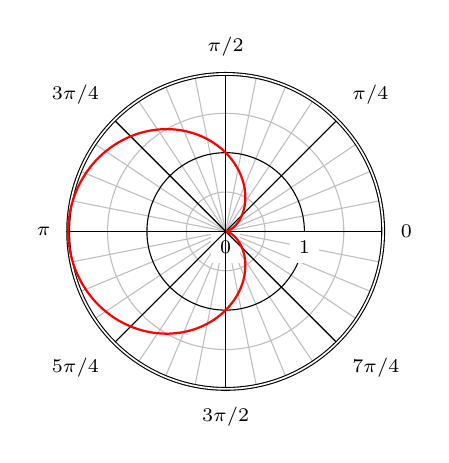
\begin{tikzpicture}[>=latex]

% Draw the lines at multiples of pi/12
\foreach \ang in {0,...,31} {
  \draw [lightgray] (0,0) -- (\ang * 180 / 16:2);
}

% Concentric circles and radius labels
\foreach \s in {0, 1} {
  \draw [lightgray] (0,0) circle (\s + 0.5);
  \draw (0,0) circle (\s);
  \node [fill=white] at (\s, 0) [below] {\scriptsize $\s$};
}

% Add the labels at multiples of pi/4
\foreach \ang/\lab/\dir in {
  0/0/right,
  1/{\pi/4}/{above right},
  2/{\pi/2}/above,
  3/{3\pi/4}/{above left},
  4/{\pi}/left,
  5/{5\pi/4}/{below left},
  7/{7\pi/4}/{below right},
  6/{3\pi/2}/below} {
  \draw (0,0) -- (\ang * 180 / 4:2);
  \node [fill=white] at (\ang * 180 / 4:2.1) [\dir] {\scriptsize $\lab$};
}

% The double-lined circle around the whole diagram
\draw [style=double] (0,0) circle (2);

\draw [thick,color=red,domain=0:2*pi,samples=200,smooth] plot (xy polar cs:angle=\x r,radius= {1-cos(\x r)});

\end{tikzpicture}
\caption*{A cardioid. \textit{TikZ code adapted from \href{https://tex.stackexchange.com/users/9668/alexwlchan}{alexwlchan} on TeX Stack Exchange}}
\end{figure}

It appears in a myriad of places (see \href{https://en.wikipedia.org/wiki/Cardioid#Properties}{Wikipedia}),
including in the Mandelbrot Set fractal and in the sensitivity patterns of some microphones.
I wanted to know its representation in Cartesian coordinates, with $y$ as a function of $x$.
(I don't remember my inital motivation for this project.
Likely I thought it would just be a fun exercise.)
After a fairly long process, I arrived at the answer,
\[y = \pm\sqrt{\frac{1\pm\sqrt{1-4x}}{2}-x-x^2},\]
where the two $\pm$ signs can vary independently.
A large number of terms canceled out near the end,
so I applied principles above
in he hope of finding a shorter derivation.\\

\textit{Note: what follows is less rigorousness and more of a thought process and intuition.
  Both have their place in math, and although we rely on the former to verify theorems,
  the latter is often responsible for coming up with them in the first place.\\
}

First of all, the first term inside the large square root (call it $z$) looks like the quadratic formula,
suggesting that it could be the root(s) of a quadratic equation.
The individual terms within $z$ can be mapped to those in the formula, giving
$-b=1$, $b^2-4ac=1-4x$, $2a=2$.
Solving for the coefficients yields $a=1$, $b=-1$, and $c=x$.
Thus, in the shortest ``ideal derivation'', there might be an equation
\[z^2-z+x=0\]
which we have to solve with the quadratic formula.
How would we arrive at $z$ during the ideal derivation, though?
We can isolate $z$ from the final answer by squaring and adding $x^2+x$, yielding
\[y^2+x^2+x=z.\]
At first, this doesn't look like much.
Looking back at the original polar formula
suggests no obvious way to get there
(or to $z^2-z+x=0$, for that matter)---until we recognize that $x^2+y^2=r^2$.
Substituting this into the previous equation yields
\[r^2+x=z.\]
The next epiphany comes when we see that this and $z^2-z+x=0$ can be rearranged to look almost identical:
\[r^2=z-x, z^2=z-x,\]
revealing the true identity of $z$ as $r$ all along
(ignoring a potential $\pm$)!
By substituting $r$ for $z$, we can write a single equation from which everything thus far (with $r$ in place of $z$) can be derived:
\[r^2-r+x=0.\]
The final step in this process (and thus the first step in the ideal derivation)
is to obtain this formula from the original $r=1-\cos\theta$.
Somehow, we need to eliminate $\cos\theta$ and introduce $x$.
For that, we refer to the identity $\cos\theta=x/r$
and recognize that multiplying both sides of the original formula by $r$
will achieve the desired effect.\\

After all of that backwards work, the derivation we find is as follows:
\begin{align}
\text{The polar equation of the cardioid is: } & r = 1-\cos(\theta) \\
\text{Multiplying both sides of (1) by } r \text{: } & r^2 = r-x \\
\text{Rearranging (2) to obtain a quadratic equation: } & r^2-r+x = 0 \\
\text{Solving (3) for } r \text{ in terms of } x \text{ with the quadratic formula: } & r = \frac{1\pm\sqrt{1-4x}}{2} \\
\text{Substituting } x^2+y^2 \text{ for } r^2 \text{ in (2): } & x^2+y^2 = r-x \\
\text{Rearranging (5) to solve for } y^2 \text{ in terms of } r \text{ and } x \text{: } & y^2 = r-x-x^2 \\
\text{Substituting } r \text{ from (4) into (6): } & y^2 = \frac{1\pm\sqrt{1-4x}}{2}-x-x^2\\
\text{Solving (7) for } y \text{ in terms of } x \text{: } & y = \pm\sqrt{\frac{1\pm\sqrt{1-4x}}{2}-x-x^2}
\end{align}

What I love about this derivation is that I'm almost sure that it can't be made any shorter.
Every part of the answer has a clear origin in some step of the derivation, and nothing seems to cancel out by chance.\\

Another place where the second principle applies includes the Gaussian integral
\[\int_{x=-\infty}^{\infty}e^{-x^2}dx=\sqrt{\pi},\]
whose derivation begins by squaring the left side (hence the square root)
and uses polar coordinates (hence the $\pi$).
Also, the fact that objects fall at the same speed toward Earth
suggested the theory of general relativity (GR)
over Newtonian gravity, where the mass term ``coincidentally'' cancels out.

\end{document}
